% ---------------------------------------------------------------
% TEMPLATE TCC1 - SENAC SANTO AMARO
% ---------------------------------------------------------------
% Trabalho de Conclusão de Curso 1
% Elaborado para apresentação da proposta inicial do TCC
% Estrutura: 4 capítulos (Introdução, Revisão Bibliográfica,
%            Desenvolvimento, Referências Bibliográficas)
%
% ARQUIVO RECONSTRUÍDO A PARTIR DO PDF COMPILADO (o codespace
% original foi perdido). Pontos que exigem atenção de Gabriel
% estão marcados com comentários "% TODO(Gabriel): ...".
% ---------------------------------------------------------------

\documentclass[
    12pt,                % tamanho da fonte
    openright,           % capítulos começam em página ímpar
    oneside,             % para impressão em apenas um lado do papel
    a4paper,             % tamanho do papel
    english,             % idioma adicional
    brazil               % idioma principal
]{abntex2}

% ---------------------------------------------------------------
% PACOTES
% ---------------------------------------------------------------
\usepackage{lmodern}                % Fonte Latin Modern
\usepackage[T1]{fontenc}            % Seleção de códigos de fonte
\usepackage[utf8]{inputenc}         % Codificação do documento
\usepackage{lastpage}               % Usado pela Ficha catalográfica
\usepackage{indentfirst}            % Indenta o primeiro parágrafo
\usepackage{color}                  % Controle de cores
\usepackage{graphicx}               % Inclusão de gráficos
\usepackage{microtype}              % Melhorias de justificação
\usepackage{float}                  % Para posicionamento de figuras
\usepackage{booktabs}               % Tabelas profissionais
\usepackage{multirow}               % Células mescladas em tabelas
\usepackage{longtable}              % Tabelas longas
\usepackage{amsmath,amssymb}        % Símbolos matemáticos
\usepackage{pgfgantt}               % Diagramas de Gantt
\usepackage{tikz}                   % Diagramas (pipeline, quadrante)
\usetikzlibrary{arrows.meta,positioning,calc}
\usepackage[brazilian,hyperpageref]{backref}  % Páginas com citações
\usepackage[alf]{abntex2cite}       % Citações ABNT
\usepackage{tabularx}                % Tabelas com largura automática

% ---------------------------------------------------------------
% CONFIGURAÇÕES DO PDF
% ---------------------------------------------------------------
\makeatletter
\hypersetup{
    pdftitle={\@title},
    pdfauthor={\@author},
    pdfsubject={TCC1 - SENAC Santo Amaro},
    pdfcreator={LaTeX with abnTeX2},
    pdfkeywords={tcc}{senac}{santo amaro}{trabalho de conclusão},
    colorlinks=true,        % false: links em caixas; true: links coloridos
    linkcolor=blue,         % cor dos links internos
    citecolor=blue,         % cor dos links para bibliografia
    filecolor=magenta,      % cor dos links para arquivos
    urlcolor=blue,
    bookmarksdepth=4
}
\makeatother

% ---------------------------------------------------------------
% CONFIGURAÇÕES DE APARÊNCIA DO PDF FINAL
% ---------------------------------------------------------------
\definecolor{blue}{RGB}{41,5,195}

% ---------------------------------------------------------------
% INFORMAÇÕES DO DOCUMENTO
% ---------------------------------------------------------------
\titulo{Análise de sensibilidade de um RNN para previsão de estoque hospitalar crítico}
\autor{Gabriel Brandão Vechani de Freitas}
\local{São Paulo}
\data{2025}
\orientador{Prof. Douglas Baquião}
% \coorientador{Prof. Nome do Coorientador} % Descomente se houver coorientador

\instituicao{%
  SENAC -- Serviço Nacional de Aprendizagem Comercial
  \par
  Unidade Santo Amaro
  \par
  Curso de Ciência da Computação
}

\tipotrabalho{Trabalho de Conclusão de Curso I}

\preambulo{Proposta de Trabalho de Conclusão de Curso apresentado ao SENAC Santo Amaro como requisito parcial para aprovação na disciplina de TCC1 do curso de Ciência da Computação.}

% ---------------------------------------------------------------
% COMPILA O ÍNDICE
% ---------------------------------------------------------------
\makeindex

% ---------------------------------------------------------------
% INÍCIO DO DOCUMENTO
% ---------------------------------------------------------------
\begin{document}

% Seleciona o idioma do documento
\selectlanguage{brazil}

% Retira espaço extra obsoleto entre as frases
\frenchspacing

% ---------------------------------------------------------------
% ELEMENTOS PRÉ-TEXTUAIS
% ---------------------------------------------------------------
\pretextual

% ---------------------------------------------------------------
% CAPA
% ---------------------------------------------------------------
\imprimircapa

% ---------------------------------------------------------------
% FOLHA DE ROSTO
% ---------------------------------------------------------------
\imprimirfolhaderosto

% ---------------------------------------------------------------
% RESUMO
% ---------------------------------------------------------------
\begin{resumo}
Este documento apresenta a proposta inicial do Trabalho de Conclusão de Curso (TCC1)
desenvolvido no SENAC Santo Amaro. O objetivo deste trabalho é [descrever brevemente
o objetivo principal do TCC]. A justificativa para este estudo baseia-se em [descrever
brevemente a justificativa]. A revisão bibliográfica abrange [mencionar os principais tópicos].
Como solução proposta, pretende-se [descrever brevemente a solução]. Este trabalho está
organizado em três capítulos que apresentam a introdução ao tema, a revisão bibliográfica
que fundamenta a pesquisa, o desenvolvimento com a solução proposta e o cronograma de
trabalho, seguidos das referências bibliográficas.

\vspace{\onelineskip}

\noindent
\textbf{Palavras-chave}: palavra1. palavra2. palavra3. palavra4. palavra5.
\end{resumo}

% ---------------------------------------------------------------
% LISTA DE ILUSTRAÇÕES
% ---------------------------------------------------------------
% \pdfbookmark[0]{\listfigurename}{lof}
% \listoffigures*
% \cleardoublepage

% ---------------------------------------------------------------
% LISTA DE TABELAS
% ---------------------------------------------------------------
% \pdfbookmark[0]{\listtablename}{lot}
% \listoftables*
% \cleardoublepage

% ---------------------------------------------------------------
% SUMÁRIO
% ---------------------------------------------------------------
\pdfbookmark[0]{\contentsname}{toc}
\tableofcontents*
\cleardoublepage

% ---------------------------------------------------------------
% ELEMENTOS TEXTUAIS
% ---------------------------------------------------------------
\textual

% ===============================================================
% CAPÍTULO 1 - INTRODUÇÃO
% ===============================================================
\chapter{Introdução}
\label{cap:introducao}

O gerenciamento de estoques é de grande importância para garantir a qualidade e a eficiência nos procedimentos hospitalares, tendo destaque significativo para a qualidade no atendimento e execução de processos. Para os hospitais, os estoques desempenham um papel fundamental, pois viabilizam a prestação de serviços aos pacientes, e principalmente, para a assistência. Ao realizar acompanhamentos de forma lógica e estratégica há uma tendência de o nível de prejuízos e desvios ser inferior. Para que a empresa ou instituição alcance um bom desempenho, é necessário, principalmente, o acompanhamento das rotinas executadas diariamente e a auditoria dos processos de estoque \citeonline{Hiaretto2021}. Uma má gestão da cadeia de abastecimento pode resultar em excesso de insumos, custos fora do orçamento e falta de itens essenciais para o atendimento. Por isso, é essencial administrar e controlar as entradas e saídas de insumos necessários para o atendimento nas instituições, mantendo o funcionamento das operações, mas com foco em menor estoque possível. Neste contexto, a instituição é desafiada cotidianamente a manter a previsibilidade de compra e consumo para que não haja desperdícios e nem falta \citeonline{Paulo2024}.

Com o aumento da complexidade dos sistemas de saúde e da demanda por insumos hospitalares, o planejamento de estoques se torna um grande desafio enfrentado pelas instituições de saúde na atualidade, sendo capaz de criar gargalos nos processos e procedimentos dessas instituições. Em um ambiente em que a escassez de recursos e a pressão assistencial são constantes, em conjunto com a imprevisibilidade da demanda, potencializada por eventos epidemiológicos, sazonalidades e picos de ocupação, a previsibilidade e a precisão operacional deixaram de ser diferenciais e tornaram-se vitais. Para \citeonline{Thiago2025}, é justamente nesse ponto que a Inteligência Artificial (IA) vem assumindo um papel transformador, oferecendo um novo patamar de precisão e eficiência na operação logística hospitalar.

Tendo isso como base, este trabalho tem como foco analisar a aplicação de uma Rede Neural Recorrente (RNN) na previsão da demanda de itens críticos em estoques hospitalares, com destaque na análise de sensibilidade do modelo de aprendizado de máquina, realizando variações nos parâmetros de entrada observando sua relevância no contexto aplicado medido com SHAP e LIME. Tendo como escolha de arquitetura a Long Short-Term Memory (LSTM), devido à sua capacidade de aprender dependências de longo prazo em dados sequenciais, com uso de camada de memória. Sendo amplamente aplicável em estoques hospitalares, devido às suas características de demanda por insumos, que podem ser influenciadas por sazonalidades, surtos epidemiológicos e variações no atendimento. O objetivo é compreender se esse tipo de modelo pode contribuir no aprimoramento da eficiência no planejamento de estoques em hospitais, auxiliando na redução de danos tanto por excesso quanto por falta de insumos.

% ---------------------------------------------------------------
\section{Contexto}
\label{sec:contexto}

Uma abordagem promissora reside na aplicação de técnicas de Deep Learning (DL), que têm demonstrado potencial para otimizar os processos de gestão da cadeia de abastecimento. Alguns estudos têm explorado a utilização de algoritmos de Machine Learning (ML) para resolver problemas de previsão de demanda, apresentando assim alternativas para melhorar a eficiência e a rentabilidade das cadeias de produção farmacêuticas e hospitalares \citeonline{SIERRAESPINEL20252791}. No entanto, a aplicação de Redes Neurais Recorrentes (RNN) para previsão de demanda em estoques hospitalares ainda é um campo pouco explorado, especialmente no que diz respeito à análise de sensibilidade do modelo a variações nos parâmetros de entrada.

Os itens críticos hospitalares, como os medicamentos essenciais, os materiais cirúrgicos e os consumíveis de suporte à vida exigem um elevado nível de controle, pois a sua indisponibilidade pode levar à interrupção de procedimentos, ao aumento do tempo de internamento ou até a riscos para a vida dos pacientes. Apesar da importância destes itens, muitos sistemas de gestão continuam a utilizar métodos tradicionais de previsão, como médias históricas ou modelos estatísticos simples, que nem sempre conseguem capturar os padrões complexos e dinâmicos da procura.

As RNN têm vasta capacidade para lidar com séries temporais, aprendendo padrões temporais e melhorando a precisão das previsões \citeonline{AGARWAL2024979}. No entanto, no contexto hospitalar, a sua utilização com este objetivo não está muito difundida, principalmente na análise de sensibilidade aos parâmetros.

% ---------------------------------------------------------------
\section{Justificativa}
\label{sec:justificativa}

A previsão de demanda por insumos críticos em ambientes hospitalares apresenta desafios particulares, decorrentes da natureza temporal, variável e muitas vezes imprevisível desse tipo de consumo. Métodos tradicionais, como médias históricas e modelos estatísticos simples, mostram-se limitados na captura dos padrões dinâmicos que caracterizam essas séries, o que motiva a investigação de técnicas de aprendizado de máquina mais adequadas a esse cenário \citeonline{math14050838}. Nesse contexto, este trabalho propõe a aplicação de uma RNN com arquitetura LSTM para a previsão de estoques hospitalares críticos, com ênfase na análise de sensibilidade do modelo frente a variações em seus parâmetros de entrada, buscando compreender de forma sistemática como tais variações influenciam seu desempenho preditivo.

Do ponto de vista acadêmico, embora as RNNs e a arquitetura LSTM sejam amplamente investigadas em tarefas de previsão de séries temporais, sua aplicação ao gerenciamento de estoques hospitalares ainda é pouco explorada na literatura, conforme evidenciado pela escassez de estudos identificados nas bases consultadas que combinam esses dois eixos. Mais incipiente ainda é a investigação sobre o impacto que variações nos parâmetros de entrada exercem sobre o desempenho preditivo nesse domínio específico, lacuna observada nos trabalhos relacionados analisados nesta pesquisa, que avaliam o desempenho de modelos LSTM sem submetê-los a perturbações controladas em suas entradas. Compreender esse comportamento é relevante porque dados hospitalares estão frequentemente sujeitos a ruídos, registros incompletos e oscilações abruptas decorrentes de eventos epidemiológicos, o que torna a robustez do modelo um critério tão importante quanto sua acurácia média. Assim, este estudo contribui para preencher essa lacuna ao oferecer uma análise sistemática da sensibilidade do modelo à variabilidade dos dados, ampliando a compreensão sobre seu comportamento em cenários hospitalares reais.

Do ponto de vista profissional, a imprecisão na previsão de demanda por itens críticos impacta diretamente a operação hospitalar e gera consequências em duas frentes. Por um lado, o excesso de insumos resulta em desperdício financeiro e em risco de perda de materiais por vencimento. Por outro lado, a falta pode comprometer a continuidade de procedimentos assistenciais e colocar em risco a segurança do paciente. Uma ferramenta preditiva mais precisa e cujo comportamento seja conhecido frente a variações nos dados oferece aos gestores de saúde uma base mais sólida para a tomada de decisão, contribuindo simultaneamente para a eficiência operacional e para a qualidade do atendimento prestado.

Por fim, o uso de dados de fontes públicas para o treinamento do modelo reforça o potencial de replicabilidade e escalabilidade da abordagem proposta, tornando-a acessível a diferentes instituições de saúde, independentemente de seu porte ou infraestrutura tecnológica.

% ---------------------------------------------------------------
\section{Objetivo}
\label{sec:objetivo}

Este estudo tem como objetivo avaliar o uso de uma Rede Neural Recorrente (RNN), com arquitetura LSTM, para a previsão de demanda de itens críticos em estoques hospitalares, investigando de forma sistemática como variações controladas em seus parâmetros de entrada e hiperparâmetros impactam o desempenho preditivo do modelo.

\subsection{Objetivo principal}

Analisar a sensibilidade de um modelo LSTM aplicado à previsão de demanda de itens críticos em estoques hospitalares, mensurando o impacto de variações controladas em parâmetros de entrada (tamanho da janela temporal, presença de ruído nas séries e proporção de valores faltantes) e em hiperparâmetros estruturais (dropout, número de camadas, número de unidades e taxa de aprendizado) sobre o desempenho preditivo do modelo, avaliado por meio das métricas Erro Absoluto Médio (MAE), Raiz do Erro Quadrático Médio (RMSE) e Erro Percentual Absoluto Médio (MAPE), Erro Absoluto Escalado Médio (MASE), bem como pela variabilidade dessas métricas frente às perturbações aplicadas.

\subsection{Objetivos secundários}
\label{sec:objetivos_secundarios}

Com base no objetivo principal serão definidos os objetivos secundários, que descrevem as etapas e ações necessárias para realizar o objetivo.

\begin{enumerate}
    \item Investigar, na literatura especializada, as principais técnicas de análise de sensibilidade aplicáveis a modelos de aprendizado profundo voltados a séries temporais, identificando aquelas mais adequadas ao contexto da previsão de estoques hospitalares críticos;
    \item Selecionar e caracterizar uma base de dados pública de consumo hospitalar adequada ao escopo do estudo, descrevendo seus atributos, limitações e o tratamento necessário (limpeza, normalização e segmentação em conjuntos de treino, validação e teste) para sua utilização no treinamento do modelo;
    \item Definir o ambiente computacional de experimentação, justificando a escolha das ferramentas, bibliotecas (como TensorFlow ou PyTorch) e recursos de hardware adotados, de modo a garantir a reprodutibilidade dos experimentos e o controle sobre os fatores externos ao modelo;
    \item Implementar e treinar um modelo LSTM de referência (baseline) para previsão de demanda de itens críticos, documentando sua arquitetura, processo de treinamento e desempenho preditivo nas métricas adotadas, de modo a estabelecer um ponto de comparação para os experimentos de sensibilidade;
    \item Definir e aplicar um protocolo experimental, aplicando perturbações controladas aos parâmetros de entrada e hiperparâmetros previamente definidos e registrando, de forma sistemática, o desempenho do modelo sob cada cenário;
    \item Utilizar técnicas de análise de sensibilidade, como SHAP e LIME, para interpretar os resultados do modelo e identificar quais entradas têm maior impacto no desempenho preditivo;
    \item Analisar e discutir os resultados obtidos, identificando quais parâmetros exercem maior influência sobre o desempenho preditivo do modelo e quais cenários representam maior risco para a aplicação prática em ambientes hospitalares, apontando limitações do estudo e direções para trabalhos futuros.
\end{enumerate}

% ===============================================================
% CAPÍTULO 2 - REVISÃO BIBLIOGRÁFICA
% ===============================================================
\chapter{Revisão Bibliográfica}
\label{cap:revisao}

Esta seção tem como objetivo apresentar o embasamento teórico do trabalho, organizando os principais conceitos e temas de forma a construir uma linha de argumentação que sustente a proposta desenvolvida.

% ---------------------------------------------------------------
\section{Referencial teórico}
\label{sec:referencial}

\subsection{Gestão de Estoques em Ambientes Hospitalares}
\label{subsec:gestao_estoques}

A gestão de estoque em ambientes hospitalares é um processo crítico e essencial para garantir a continuidade e qualidade de sistemas de saúde. Como característica hospitalar é lidar com uma grande variedade de itens, que possuem data de validade, alta criticidade e demanda frequentemente variável. Nesse contexto, a falta de determinado item pode comprometer diretamente o atendimento ao paciente. Por outro lado o excesso de estoque pode resultar em desperdício e aumento de custos. Sendo assim, o sistema logístico hospitalar deve ser eficientemente planejado e coordenado, conforme relatado por \citeonline[p.~68]{Claudia2021}.

Em complemento, o uso de tecnologias e técnicas avançadas, como o aprendizado de máquina, tem se mostrado promissor para otimizar a gestão de estoques hospitalares. A capacidade de prever a demanda com maior precisão pode ajudar a reduzir tanto o excesso quanto a falta de insumos, melhorando a eficiência operacional e a qualidade do atendimento ao paciente. No entanto, a aplicação dessas técnicas ainda é um campo em desenvolvimento, especialmente no que diz respeito à análise de sensibilidade dos modelos preditivos utilizados, assim como descrito por \citeonline{SIERRAESPINEL20252791}.

\subsection{Redes Neurais Recorrentes e LSTMs para Séries Temporais}
\label{subsec:rnn_lstm}

Uma rede neural recorrente (RNN) é um tipo de rede neural projetada para processar entradas sequenciais, como séries temporais, sendo amplamente utilizada em aprendizado de máquina por sua capacidade de gerar conclusões e previsões a partir desses dados. Seu mecanismo de aprendizagem é baseado na retropropagação, adaptada para redes compostas por unidades semelhantes a neurônios. A arquitetura conta com camadas ocultas dotadas de conexões recorrentes, nas quais a saída de uma camada é realimentada como entrada para ela mesma. Esse mecanismo permite que a rede mantenha um estado interno capaz de capturar e preservar informações sobre o histórico da sequência processada, conforme descrito por \citeonline{Elman1990}. O procedimento ajusta repetidamente os pesos das conexões na rede de modo a minimizar uma medida da diferença entre o vetor de saída real da rede e o vetor de saída desejado, segundo \citeonline{Rumelhart1986}.

% TODO(Gabriel): reinserir aqui o arquivo de imagem original (diagrama de ajuste de pesos).
\begin{figure}[H]
    \centering
    \fbox{\parbox{0.75\textwidth}{\centering\vspace{2.2cm}\textit{[Reinserir imagem: diagrama de ajuste de peso entre neurônios]}\vspace{2.2cm}}}
    \caption{A imagem ilustra um sistema simples de ajuste de peso entre os neurônios, \citeonline{Rumelhart1986}}
    \label{fig:rumelhart}
\end{figure}

Podendo ser usada para previsão de demanda, classificação de texto, reconhecimento de fala, entre outros. As RNNs são capazes de capturar dependências temporais em dados sequenciais, o que as torna adequadas para tarefas como previsão de séries temporais, onde os padrões podem se estender por longos intervalos de tempo. No entanto, as RNNs tradicionais enfrentam dificuldades para aprender dependências de longo prazo devido ao problema do desvanecimento do gradiente, o que limita sua eficácia em tarefas que exigem a retenção de informações por períodos prolongados.

A arquitetura Long Short-Term Memory (LSTM) é um tipo de RNN projetada para lidar com o problema do desvanecimento do gradiente, permitindo que a rede aprenda dependências de longo prazo em dados sequenciais \citeonline{Hochreiter1997}. Diferentemente de uma RNN tradicional, cada célula LSTM mantém um estado de célula (cell state), uma memória de longo prazo que percorre a sequência e cujo conteúdo é regulado por três mecanismos de controle de fluxo denominados portas (gates): a porta de entrada (input gate), que define quais novas informações são incorporadas ao estado de célula; a porta de esquecimento (forget gate), que determina quais informações do estado anterior devem ser descartadas; e a porta de saída (output gate), que controla qual parcela do estado é exposta como saída da célula no instante corrente.

% TODO(Gabriel): reinserir aqui o arquivo de imagem original (ilustração da célula LSTM).
\begin{figure}[H]
    \centering
    \fbox{\parbox{0.75\textwidth}{\centering\vspace{2.2cm}\textit{[Reinserir imagem: ilustração da arquitetura LSTM]}\vspace{2.2cm}}}
    \caption{Simples ilustração da arquitetura LSTM, representando a estrutura de memória e os mecanismos de controle de fluxo, \citeonline{Hochreiter1997}}
    \label{fig:lstmcell}
\end{figure}

É essa regulação seletiva manter, atualizar ou descartar informações que permite à LSTM preservar dependências por períodos prolongados sem que o gradiente se dissipe ao longo do tempo, tornando-a especialmente adequada a tarefas como a previsão de séries temporais, nas quais os padrões podem se estender por longos intervalos. Cabe registrar que a formulação original \citeonline{Hochreiter1997} contemplava apenas as portas de entrada e de saída, tendo a porta de esquecimento sido introduzida posteriormente por \citeonline{Gers2000}, configuração que corresponde à forma da arquitetura amplamente utilizada na atualidade. No domínio deste estudo a previsão de demanda em estoques hospitalares essa capacidade de capturar padrões temporais complexos é crucial para melhorar a precisão das previsões e otimizar o gerenciamento de suprimentos.

\subsection{Previsão de Ruptura e Níveis de Estoque}
\label{subsec:ruptura}

A previsão de ruptura de estoque (stockout), refere-se à antecipação do momento em que o nível de um item disponível torna-se insuficiente para atender à demanda. Em contextos hospitalares, esse evento é particularmente crítico, pois pode comprometer a continuidade de procedimentos assistenciais, ou até mesmo colocar em risco a segurança do paciente. Para mitigar esse risco, a literatura de gestão de operações estabelece dois conceitos fundamentais que orientam a política de reposição: o estoque de segurança (safety stock), entendido como a quantidade adicional mantida em estoque para absorver variações na demanda e nos prazos de entrega, e o ponto de pedido (reorder point), definido como o nível de estoque a partir do qual uma nova ordem de reposição deve ser emitida, calculado tradicionalmente como a soma entre a demanda esperada durante o tempo de espera e o estoque de segurança. A precisão desses parâmetros depende diretamente da qualidade da previsão de demanda subjacente, uma vez que estimativas imprecisas geram tanto excesso de estoque, com custos financeiros e risco de vencimento, quanto rupturas, com prejuízos operacionais e clínicos.

Tradicionalmente, esses cálculos têm sido realizados por meio de fórmulas estatísticas que assumem distribuições conhecidas da demanda e do tempo de espera, o que pode ser limitante em ambientes hospitalares marcados por demandas intermitentes, sazonalidades e eventos epidemiológicos. Para superar essas restrições, estudos recentes têm proposto integrar modelos de aprendizado profundo, especialmente arquiteturas recorrentes como a LSTM, ao processo de previsão de demanda que alimenta o cálculo do estoque de segurança e do ponto de pedido. Trabalhos como o de \citeonline{SEYEDAN2023100024} demonstram que abordagens baseadas em Aprendizado em Conjunto (ensemble) com LSTM podem melhorar a acurácia das previsões e, consequentemente, permitir a definição dinâmica dos níveis de estoque sob diferentes cenários de tempo de espera. Entretanto, conforme apontam \citeonline{math14050838}, em séries com baixa razão sinal-ruído, modelos LSTM treinados com função de perda quadrática, Erro Quadrático Médio (MSE), tendem a suavizar picos de demanda, o que pode resultar em subestimação sistemática e em cálculos enviesados do estoque de segurança, aumentando o risco de ruptura. Esse comportamento reforça a necessidade de avaliar não apenas a acurácia média do modelo, mas também sua sensibilidade frente a variações nas entradas, especialmente quando suas previsões alimentam decisões logísticas com impacto direto sobre a operação hospitalar.

\subsection{Análise de Sensibilidade e Robustez em Modelos de IA}
\label{subsec:sensibilidade}

A análise de sensibilidade em modelos de inteligência artificial consiste no estudo sistemático de como variações controladas em parâmetros ou entradas do modelo afetam suas saídas, sendo um instrumento essencial para avaliar a estabilidade, a interpretabilidade e a confiabilidade de soluções baseadas em aprendizado profundo. No contexto de redes neurais, essa análise pode ser conduzida em duas frentes principais: a sensibilidade a hiperparâmetros, que examina o impacto de escolhas estruturais, como número de camadas, taxa de aprendizado, função de ativação e dimensão de janela temporal sobre o desempenho preditivo \citeonline{novello2022}; e a sensibilidade aos dados de entrada, que avalia a resposta do modelo frente a perturbações aplicadas às variáveis da série temporal, sejam elas ruídos, valores faltantes ou alterações em variáveis específicas \citeonline{wang2024}. Já o conceito de robustez é frequentemente associado à capacidade do modelo de manter desempenho estável diante dessas perturbações, sendo, portanto, uma propriedade verificada a partir da análise de sensibilidade. Em séries temporais, essas avaliações são particularmente relevantes, pois pequenas variações em parâmetros como tamanho da janela de entrada ou taxa de regularização podem alterar significativamente a capacidade do modelo de capturar padrões temporais complexos.

Entre as técnicas mais utilizadas para conduzir esse tipo de análise, destacam-se métodos baseados em perturbação direta das entradas com medição da variação na saída, conforme descrito por \citeonline{guan2024}, índices estatísticos como o critério HSIC (Hilbert-Schmidt Independence Criterion) aplicado à exploração do espaço de hiperparâmetros, conforme citado por \citeonline{novello2022}, e abordagens de explicabilidade como SHAP (SHapley Additive exPlanations). Quando aplicadas a modelos LSTM, essas técnicas permitem identificar quais janelas temporais e quais variáveis exercem maior influência sobre a previsão, fornecendo subsídios para a interpretação e o aprimoramento do modelo, conforme explicado por \citeonline{Divyani2025}. Além disso, estudos de ablação, em que componentes do modelo ou subconjuntos de features são removidos para observar o impacto no desempenho, complementam a avaliação ao expor possíveis dependências críticas. No contexto da previsão de estoques hospitalares, a aplicação dessas técnicas é especialmente pertinente, pois os dados costumam apresentar ruídos, registros incompletos e padrões irregulares decorrentes de eventos epidemiológicos, fatores que tornam a análise de sensibilidade um requisito tanto técnico quanto operacional para garantir confiabilidade nas decisões logísticas baseadas no modelo.

\subsection{Pré-processamento de Séries Temporais e Imputação de Dados}
\label{subsec:preprocessamento}

O pré-processamento de séries temporais compreende um conjunto de etapas fundamentais que precedem a modelagem preditiva, incluindo normalização, verificação de estacionariedade, remoção de outliers e decomposição da série em seus componentes estruturais. Em séries temporais reais, a não estacionariedade é um desafio recorrente, uma vez que propriedades estatísticas como média e variância variam ao longo do tempo, dificultando a generalização de modelos de aprendizado profundo, como citado por \citeonline{Wang2026survey}. Técnicas como diferenciação, decomposição sazonal e normalização por instância têm sido amplamente utilizadas para mitigar esses efeitos, permitindo que os modelos capturem padrões temporais com maior fidelidade. A decomposição STL (Seasonal-Trend decomposition using LOESS) destaca-se por sua versatilidade e robustez, sendo aplicada como etapa de pré-processamento em combinação com modelos de aprendizado de máquina para melhorar o desempenho preditivo, como demonstrado em \citeonline{Bandara2021}.

A imputação de dados ausentes é etapa crítica no tratamento de séries temporais, especialmente em contextos onde falhas de registro eletrônico são frequentes. Relações temporais são afetadas quando valores ausentes são simplesmente ignorados, pois padrões sazonais podem ser obscurecidos, tornando imprescindível a adoção de estratégias de imputação mais sofisticadas, mostrado por \citeonline{Poette2026}. Além das abordagens tradicionais como média, mediana e LOCF (last observation carried forward), modelos de aprendizado profundo têm demonstrado crescente capacidade para imputação de séries temporais multivariadas, com redes neurais recorrentes e arquiteturas baseadas em Transformers se destacando nos benchmarks recentes, demonstrado em \citeonline{Wang2025imputation}. A escolha do método de imputação deve considerar o mecanismo de ausência dos dados (MCAR, MAR ou MNAR) e a estrutura temporal da série, pois abordagens inadequadas podem introduzir viés sistemático nos resultados, demonstrado por \citeonline{Haneuse2021}.

\subsection{Métricas de Desempenho e Erro}
\label{subsec:metricas}

A avaliação quantitativa de modelos preditivos em séries temporais depende da escolha criteriosa de métricas de erro que reflitam adequadamente a natureza do problema. As métricas mais comuns incluem o Erro Absoluto Médio (MAE), a Raiz do Erro Quadrático Médio (RMSE) e o Erro Percentual Absoluto Médio (MAPE): o RMSE é preferido quando erros maiores devem ser penalizados com mais intensidade, enquanto o MAPE expressa o erro como percentual dos valores reais, facilitando a comparação entre séries de diferentes escalas, como citado em \citeonline{Makridakis2022}. Cada métrica apresenta limitações específicas: o MAPE é problemático quando os valores reais se aproximam de zero, situação frequente em demandas intermitentes, e apresenta assimetria ao penalizar mais fortemente as superestimações do que as subestimações.

O MASE (Erro Médio Absoluto Escalonado) tem ganhado espaço como alternativa robusta, especialmente por sua capacidade de comparar desempenhos entre séries de diferentes escalas sem ser afetado por valores nulos, sendo considerado superior ao benchmark ingênuo quando seu valor é inferior a 1, citado em \citeonline{Makridakis2022}. Em contextos aplicados à saúde, a escolha da métrica deve também considerar as implicações operacionais dos erros: superestimações e subestimações da demanda hospitalar têm custos assimétricos, o excesso de provisão gera desperdício de recursos, enquanto a subestimação compromete a qualidade do atendimento \citeonline{Vollmer2021}. A avaliação de precisão não deve se restringir à etapa final da modelagem, mas estar integrada ao longo de todo o fluxo de trabalho, incluindo seleção de modelos, ajuste de hiperparâmetros e monitoramento contínuo em produção.

\subsubsection{Erro Absoluto Médio (MAE)}
\label{subsec:mae}

\begin{equation}
\text{MAE} = \frac{1}{n}\sum_{i=1}^{n}\left|y_i - \hat{y}_i\right|
\end{equation}

Mede a média dos valores absolutos dos erros, onde $y_i$ é o valor real, $\hat{y}_i$ é o valor previsto e $n$ é o número de observações. Por usar o valor absoluto, todos os erros têm o mesmo peso, independentemente do sinal. O resultado fica na mesma unidade da variável original, o que facilita a interpretação. É robusto a outliers, já que não eleva os erros ao quadrado.

\subsubsection{Raiz do Erro Quadrático Médio (RMSE)}
\label{subsec:rmse}

\begin{equation}
\text{RMSE} = \sqrt{\frac{1}{n}\sum_{i=1}^{n}\left(y_i - \hat{y}_i\right)^2}
\end{equation}

É a raiz quadrada da média dos erros elevados ao quadrado. Como os erros são elevados ao quadrado antes de serem somados, o RMSE penaliza mais fortemente os erros grandes, ou seja, é mais sensível a outliers do que o MAE. A raiz quadrada final devolve o resultado à mesma unidade da variável original. Sempre vale a relação RMSE $\geq$ MAE.

\subsubsection{Erro Percentual Absoluto Médio (MAPE)}
\label{subsec:mape}

\begin{equation}
\text{MAPE} = \frac{100\%}{n}\sum_{i=1}^{n}\left|\frac{y_i - \hat{y}_i}{y_i}\right|
\end{equation}

Expressa o erro como uma porcentagem média em relação aos valores reais, o que o torna adimensional e útil para comparar o desempenho entre conjuntos de dados de escalas diferentes. Tem duas limitações importantes: fica indefinido quando algum $y_i = 0$ e tende a penalizar de forma assimétrica, pesando mais as previsões que superestimam do que as que subestimam.

\subsubsection{Erro Absoluto Escalado Médio (MASE)}
\label{subsec:mase}

Para a fórmula, precisamos definir duas quantidades. O erro do modelo no instante $i$ é:

\begin{equation}
e_i = y_i - \hat{y}_i
\end{equation}

E o erro médio absoluto do preditor ingênuo sazonal (naive com período $m$), calculado in-sample sobre $T$ observações de treinamento, é:

\begin{equation}
\text{MAE}_{\text{naive}} = \frac{1}{T-m}\sum_{t=m+1}^{T}\left|y_t - y_{t-m}\right|
\end{equation}

O MASE é então definido como \cite{Hyndman2006}:

\begin{equation}
\text{MASE} = \frac{1}{n}\sum_{i=1}^{n}\frac{\left|e_i\right|}{\text{MAE}_{\text{naive}}} = \dfrac{\dfrac{1}{n}\displaystyle\sum_{i=1}^{n}\left|y_i - \hat{y}_i\right|}{\dfrac{1}{T-m}\displaystyle\sum_{t=m+1}^{T}\left|y_t - y_{t-m}\right|}
\end{equation}

onde $m$ é o período sazonal da série e $T$ é o número de observações de treinamento. Por ser adimensional e normalizado por um benchmark bem definido, o MASE resolve as duas limitações centrais do MAPE: permanece definido mesmo quando $y_i = 0$, o que é relevante em contextos hospitalares onde itens de baixa rotatividade podem registrar demanda nula em determinados períodos, e não apresenta a assimetria de penalização observada naquela métrica. Um valor MASE $<$ 1 indica que o modelo supera o preditor ingênuo sazonal; um valor MASE $>$ 1 indica desempenho inferior a ele.

\subsection{Particularidades da Demanda Hospitalar}
\label{subsec:particularidades}

A demanda hospitalar apresenta características estruturais que a distinguem de outras séries temporais de previsão, impondo desafios específicos à modelagem. Dados de sistemas de emergência exibem forte sazonalidade e não linearidade em períodos normais, enquanto períodos de pico seguem um padrão trifásico: estresse inicial de recursos, expansão de capacidade e recuperação do sistema, exigindo abordagens capazes de capturar essas dinâmicas operacionais distintas. Além da variação sazonal anual e semanal, fatores exógenos como condições climáticas, surtos epidemiológicos, feriados e eventos locais exercem influência significativa sobre o fluxo de pacientes, tornando essencial a incorporação de variáveis externas nos modelos preditivos \citeonline{Petsis2022}.

A previsão precisa de chegadas de pacientes em prontos-socorros é crítica para o planejamento de capacidade e para a tomada de decisão clínica, sendo que modelos de inteligência artificial, em especial de aprendizado de máquina e aprendizado profundo, têm demonstrado desempenho promissor em relação às abordagens tradicionais de séries temporais \citeonline{Petsis2022}. A alta variabilidade inerente à demanda de emergência, a presença de dados ausentes em registros eletrônicos de saúde e a heterogeneidade entre unidades hospitalares são fatores que demandam metodologias robustas e adaptáveis ao contexto local \citeonline{Poette2026}.

\subsection{Medicamentos para doenças respiratórias}
\label{subsec:respiratorios}

Os medicamentos destinados ao tratamento de doenças respiratórias constituem um exemplo representativo de item crítico em estoques hospitalares, na medida em que reúnem as duas características discutidas anteriormente: elevada criticidade assistencial e demanda fortemente influenciada por fatores sazonais e epidemiológicos. Conforme apontado na seção~\ref{subsec:particularidades}, a demanda hospitalar é particularmente sensível a variáveis exógenas como condições climáticas e surtos epidemiológicos \citeonline{Petsis2022}. Esse vínculo se manifesta diretamente no consumo de medicamentos: a literatura de previsão de demanda farmacêutica reconhece que os padrões de consumo são moldados por ciclos sazonais de doenças e pelo surgimento de novas enfermidades, fatores que dificultam o uso de modelos estatísticos tradicionais e motivam abordagens baseadas em aprendizado profundo \citeonline{Chen2026}. As infecções respiratórias ilustram esse padrão de maneira clara, pois sua incidência se intensifica nos meses frios, elevando de forma significativa os atendimentos em prontos-socorros e as internações hospitalares, sobretudo entre populações vulneráveis como crianças, idosos e portadores de doenças crônicas.

No Brasil, vírus respiratórios como o influenza e o vírus sincicial respiratório (VSR) apresentam circulação tipicamente concentrada no outono e no inverno, ainda que com variações regionais relevantes \citeonline{SBIm2026}. Esse comportamento sazonal, contudo, não é perfeitamente regular: a pandemia de COVID-19 alterou a sazonalidade esperada de vírus respiratórios como o VSR, que passou a circular também fora dos períodos tradicionais, gerando ondas atípicas de demanda. No campo da previsão de demanda hospitalar de medicamentos, esse tipo de evento é formalmente tratado como ponto de mudança: padrões não estacionários que mudam abruptamente de patamar, frequentemente associados a eventos como uma pandemia, e que \citeonline{Xu2025} identificaram afetar parcela expressiva dos itens de maior movimentação em uma farmácia hospitalar. Essa combinação de sazonalidade recorrente com episódios imprevisíveis reforça a dificuldade de previsão da demanda nesse grupo de itens.

Do ponto de vista da gestão de estoques, essas características tornam os medicamentos respiratórios um objeto especialmente adequado para investigar a aplicação de modelos preditivos baseados em séries temporais. A demanda farmacêutica hospitalar é descrita como intermitente, volátil e variável conforme a granularidade temporal e a localização dentro do hospital, o que desafia métodos tradicionais e justifica arquiteturas capazes de capturar dependências temporais complexas \citeonline{Barrow2026}. A presença simultânea de sazonalidade marcante, dependência de fatores exógenos e ocorrência de picos abruptos cria justamente o tipo de série para o qual arquiteturas recorrentes como a LSTM foram concebidas (Seção~\ref{subsec:rnn_lstm}), ao mesmo tempo em que expõe o modelo a perturbações, ruídos, oscilações e registros incompletos, os quais motivam a análise de sensibilidade proposta neste trabalho. Dessa forma, o recorte sobre medicamentos para doenças respiratórias não apenas delimita o escopo do estudo, como também oferece um cenário realista e desafiador para avaliar a robustez do modelo frente a variações em seus parâmetros de entrada.

% ---------------------------------------------------------------
\section{Metodologia da pesquisa bibliográfica}
\label{sec:metodologia_pesquisa}

A seguir são apresentados os principais tópicos que nortearam a condução desta pesquisa:

\begin{itemize}
    \item \textbf{Bases de dados consultadas}: Google Scholar, IEEE Xplore, ACM Digital Library, SciELO, Periódicos CAPES, entre outras;
    \item \textbf{Palavras-chave utilizadas}:
    \begin{itemize}
        \item ("critical inventory" OR "critical stock" OR "medical supplies" OR "hospital formulary") AND ("deep learning" OR "neural network" OR "LSTM" OR "RNN") AND ("forecasting" OR "optimization" OR "demand prediction") AND ("hospital" OR "healthcare" OR "pharmaceutical");
        \item ("LSTM" OR "GRU" OR "recurrent neural network") AND ("time series forecasting" OR "sequential prediction");
        \item ("inventory management" OR "stock forecasting" OR "demand prediction") AND ("hospital" OR "pharmacy" OR "medical supplies" OR "critical stock");
        \item ("sensitivity analysis" OR "feature importance" OR "SHAP" OR "Sobol index" OR "ablation study") AND ("neural network" OR "deep learning" OR "machine learning").
    \end{itemize}
    \item \textbf{Critérios de inclusão e exclusão}: Os critérios de inclusão adotados para a seleção dos trabalhos foram: publicações nos idiomas português e inglês; trabalhos do tipo científico, como artigos, dissertações, notícias; publicações dos últimos 5 a 6 anos, garantindo a atualidade das referências; e relevância acadêmica, priorizando trabalhos publicados em periódicos indexados, alinhados à temática central da pesquisa;
    \item \textbf{Período de abrangência}: média de 5 a 6 anos.
\end{itemize}

A pesquisa bibliográfica foi realizada nas bases Google Scholar, IEEE Xplore, ACM Digital Library, SciELO e Periódicos CAPES, entre outras, utilizando combinações de palavras-chave estruturadas em quatro eixos temáticos: gestão de estoque crítico e insumos hospitalares, redes neurais recorrentes e aprendizado profundo, previsão de demanda em ambientes de saúde, e análise de sensibilidade em modelos de aprendizado de máquina. Entre as expressões empregadas destacam-se termos como "critical inventory", "LSTM", "demand prediction", "hospital pharmacy", "SHAP" e "LIME", combinados por operadores booleanos para maior precisão na recuperação dos resultados. Foram selecionados artigos publicados predominantemente nos últimos cinco a seis anos, em português e inglês, que abordassem diretamente a aplicação de técnicas de aprendizado profundo com ênfase em arquiteturas recorrentes como LSTM e GRU na previsão e otimização de estoques críticos em contextos hospitalares e farmacêuticos. Foram excluídos trabalhos que não apresentassem relação direta com os temas centrais da pesquisa, publicações sem revisão por pares e estudos cujo foco recaísse exclusivamente sobre domínios clínicos sem interface com gestão de suprimentos ou modelagem preditiva.

% ---------------------------------------------------------------
\section{Trabalhos relacionados}
\label{sec:trabalhos_relacionados}

Nesta seção serão apresentados 3 trabalhos selecionados que têm como base o uso de redes neurais recorrentes (RNN/LSTM), aprendizado de máquina e séries temporais, além da análise crítica de seus respectivos resultados. Os trabalhos foram escolhidos seguindo os critérios citados em \ref{sec:metodologia_pesquisa}, contribuindo para a compreensão do estado da arte na área. A seguir, é apresentado um resumo individual de cada um dos trabalhos pesquisados, descrevendo seus objetivos, metodologias adotadas e os principais desafios enfrentados ao longo de seu desenvolvimento.

\subsection{Trabalho 1: Applying Deep Learning and Forecasting Techniques to the Pharmaceutical Supply Chain}

\citeonline{SIERRAESPINEL20252791} abordou o problema de melhorar o atendimento aos pacientes através da disponibilidade de medicamentos, como também contribuir para a eficácia operacional no setor da saúde. Para resolvê-lo, os autores propuseram aplicar técnicas de modelação econométrica e estratégias de aprendizagem profunda (DL), com o objetivo de mensurar e gerar previsões com uma boa precisão. A metodologia utilizada foi MLOps (Operações de Aprendizagem Automática), abrangendo princípios de desenvolvimento de software com práticas de gestão de sistemas, onde foi usado para identificação de modelos e estratégias mais adequadas. Já para o modelo econométrico ARIMA, foram utilizados critérios como o Critério de Informação de Akaike (AIC), o Critério de Informação Bayesiano (BIC) e o Critério de Informação de Hannan-Quinn (HQIC), em conjunto ao teste de Ljung-Box. E para avaliar o aprendizado profundo, foram usados o Erro Absoluto Médio (MAE), o Erro Quadrático Médio (MSE) e o Raiz do Erro Quadrático Médio (RMSE).

% TODO(Gabriel): substituir a frase abaixo pelos valores numéricos exatos (MAE, MSE, RMSE, AIC, BIC, HQIC) publicados na tabela de resultados de \citeonline{SIERRAESPINEL20252791}, para permitir comparação direta com os resultados deste trabalho.
Os resultados mostraram que os dois modelos, o econométrico ARIMA e o de aprendizado profundo (DL), possuem uma eficácia significativa para previsões de demanda de medicamentos, onde em conjunto podem oferecer uma maior precisão nas previsões, resultado demonstrado com o uso dos critérios definidos. No entanto, a solução apresenta limitações como a ausência de análise de sensibilidade nos parâmetros de entrada e a não avaliação da robustez dos modelos frente a perturbações nos dados de entrada. O presente trabalho diferencia-se por fazer uso de uma base pública, a qual será tratada para resultar em um grupo de medicamentos essenciais para o sistema de saúde, e por aplicar testes nos parâmetros de entrada para avaliar como o modelo de aprendizagem de máquina se comporta frente a essas variações.

\subsection{Trabalho 2: Predictive Data Analysis: Leveraging RNN and LSTM Techniques for Time Series Dataset}

\citeonline{AGARWAL2024979} abordou o problema de prever valores futuros de cotações no mercado de ações. Para resolvê-lo, os autores propuseram utilizar Redes Neurais Recorrentes (RNN) e Memória de Longo Prazo (LSTM) para gerar previsões a partir de um conjunto de dados, superando o problema do desvanecimento do gradiente com o uso da arquitetura LSTM. A metodologia utilizada foi estruturar a solução em módulos e classes, sendo eles:
\begin{itemize}
\item Módulo de pré-processamento de dados: inclui as funções para carregar, limpar e normalizar os dados relativos aos preços das ações;
\item Módulo de arquitetura do modelo: inclui as funções para construir os modelos RNN e LSTM;
\item Módulo de treino: inclui as funções para treinar os modelos com base nos dados históricos;
\item Módulo de previsão: inclui as funções para efetuar previsões sobre os dados de teste e avaliar o desempenho dos modelos.
\end{itemize}
Para construir os modelos, os autores utilizaram Python e as bibliotecas Keras e TensorFlow. Para normalizar os dados, foi utilizado o MinMaxScaler da biblioteca sklearn. A separação dos conjuntos de treino e teste foi de 85:15, ou seja, 85\% dos dados foram utilizados para treinar o modelo LSTM e 15\% para teste, com janelas de 100 pontos de dados. O Raiz do Erro Quadrático Médio (RMSE), as medidas R² e as métricas de acurácia foram utilizados para avaliar o desempenho dos modelos.

Os resultados mostraram que o modelo LSTM apresentou desempenho superior ao modelo RNN: o modelo RNN, após 100 épocas, obteve uma acurácia de 97,12\% nos dados de treino e de 81,01\% nos dados de teste, enquanto o modelo LSTM, aplicado ao mesmo conjunto de dados, alcançou 98,10\% nos dados de treino e 91,97\% nos dados de teste. No entanto, assim como o trabalho anterior, a solução apresenta limitações como a ausência de análise de sensibilidade nos parâmetros de entrada, a não avaliação da robustez dos modelos frente a perturbações nos dados e a aplicação restrita ao domínio financeiro, sem contemplar contextos hospitalares. O presente trabalho diferencia-se por aplicar métodos de análise de sensibilidade e avaliação da robustez em um modelo preditivo voltado à gestão de estoques hospitalares críticos.

\subsection{Trabalho 3: Performance analysis of neural network architectures for time series forecasting: A comparative study of RNN, LSTM, GRU, and hybrid models}

\citeonline{YUNITA2025103462} abordou o problema de avaliar o desempenho de nove arquiteturas de redes neurais para previsão de séries temporais, nomeadamente RNN, LSTM, GRU, RNN-LSTM, RNN-GRU, LSTM-RNN, GRU-RNN, LSTM-GRU e GRU-LSTM. Para resolvê-lo, os autores propuseram uma avaliação baseada no método de Monte Carlo (MC), com o objetivo de garantir a confiabilidade dos resultados frente à variabilidade decorrente da inicialização aleatória dos pesos. A metodologia utilizada consistiu em selecionar três conjuntos de dados nas áreas da astronomia, cuidados de saúde e maquinaria, realizar uma análise exploratória de dados (EDA) como etapa preliminar de avaliação estatística e de qualidade, implementar as diferentes arquiteturas de redes neurais e, por fim, avaliar os modelos por meio de 100 iterações de Monte Carlo, utilizando as métricas de Erro Absoluto Médio (MAE), Erro Percentual Absoluto Médio (MAPE) e Raiz do Erro Quadrático Médio (RMSE).

Os resultados mostraram que, pelo teste de Friedman, não houve diferença estatisticamente significativa entre as arquiteturas avaliadas. Esse resultado pode ter sido influenciado por fatores como a dimensão limitada da amostra, com apenas três conjuntos de dados para avaliação, e o possível mascaramento das diferenças de desempenho pelo ruído experimental. Ainda assim, os padrões de desempenho consistentes observados em todos os conjuntos de dados sugerem potenciais vantagens práticas para as arquiteturas híbridas baseadas em LSTM, especialmente as configurações LSTM-RNN e LSTM-GRU. No entanto, a solução apresenta limitações como o número reduzido de conjuntos de dados utilizados na avaliação, a ausência de investigação sobre o impacto de perturbações nos parâmetros de entrada sobre o desempenho preditivo e a não aplicação dos modelos em contextos hospitalares. O presente trabalho diferencia-se por aplicar uma análise de sensibilidade sistemática nos parâmetros de entrada de um modelo LSTM voltado à previsão de estoques hospitalares críticos, investigando como variações nesses parâmetros afetam o desempenho preditivo, parte não explorada por \citeonline{YUNITA2025103462}, que avaliam a robustez apenas em relação à inicialização aleatória dos pesos, sem considerar perturbações nos dados de entrada.

\vspace{0.3cm}
Posicionamento acadêmico dos trabalhos relacionados:

% Reconstrução do gráfico de quadrantes (figura original: posicionamento acadêmico dos
% trabalhos relacionados). Ajuste as coordenadas se desejar reposicionar os pontos.
\begin{figure}[H]
    \centering
    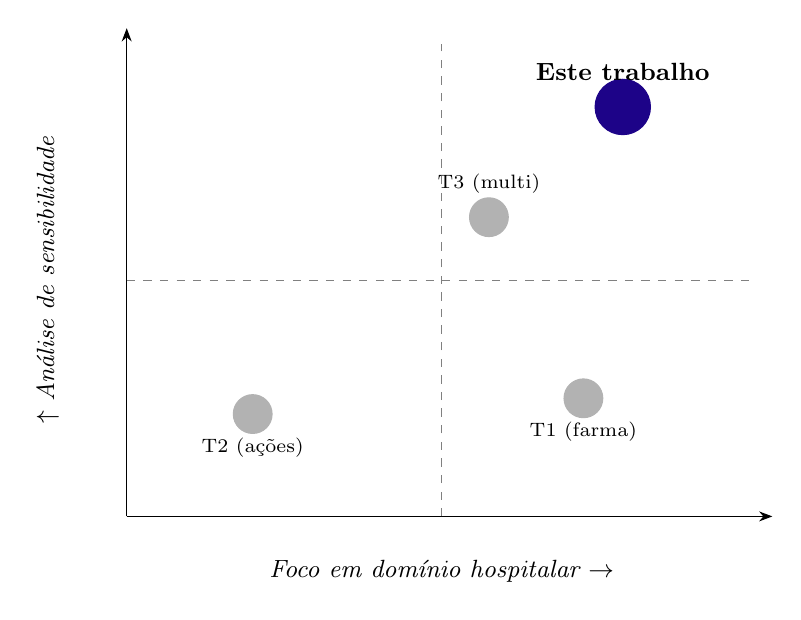
\begin{tikzpicture}[scale=1.0]
        \draw[-Stealth] (0,0) -- (8.2,0);
        \draw[-Stealth] (0,0) -- (0,6.2);
        \draw[dashed, gray] (4,0) -- (4,6);
        \draw[dashed, gray] (0,3) -- (8,3);
        \node[font=\small\itshape] at (4,-0.7) {Foco em domínio hospitalar $\rightarrow$};
        \node[font=\small\itshape, rotate=90] at (-1.0,3) {$\uparrow$ Análise de sensibilidade};
        \filldraw[gray!60] (1.6,1.3) circle (7pt);
        \node[font=\scriptsize, below=5pt] at (1.6,1.3) {T2 (ações)};
        \filldraw[gray!60] (5.8,1.5) circle (7pt);
        \node[font=\scriptsize, below=5pt] at (5.8,1.5) {T1 (farma)};
        \filldraw[gray!60] (4.6,3.8) circle (7pt);
        \node[font=\scriptsize, above=5pt] at (4.6,3.8) {T3 (multi)};
        \filldraw[blue!70!black] (6.3,5.2) circle (10pt);
        \node[font=\small\bfseries, above=6pt] at (6.3,5.2) {Este trabalho};
    \end{tikzpicture}
    \caption{A imagem ilustra o posicionamento acadêmico deste trabalho em relação aos trabalhos relacionados}
    \label{fig:posicionamento}
\end{figure}

Uma tabela comparativa ajuda a sintetizar as diferenças entre os trabalhos:

\begin{table}[htb]
    \centering
    \caption{Comparação entre trabalhos relacionados}
    \label{tab:trabalhos_relacionados}

    \begin{tabularx}{\textwidth}{p{2.8cm}|X|X|X|X}
        \toprule
        \textbf{Critério} & \textbf{Trabalho 1} & \textbf{Trabalho 2} & \textbf{Trabalho 3} & \textbf{Este trabalho} \\
        \midrule
        Objetivo
        & Previsão de demanda farmacêutica
        & Previsão de cotações de ações
        & Comparação de arquiteturas RNN, LSTM e GRU
        & Análise de sensibilidade de LSTM para estoque hospitalar crítico \\

        \midrule

        Tecnologia
        & ARIMA + DL (MLOps)
        & RNN + LSTM (Keras/TensorFlow)
        & RNN, LSTM, GRU, modelos híbridos
        & LSTM + análise de sensibilidade \\

        \midrule

        Validação
        & MAE, MSE, RMSE, AIC, BIC
        & RMSE, R², acurácia
        & MAE, MAPE, RMSE (Monte Carlo)
        & MAE, RMSE, MAPE e MASE \\

        \midrule

        Limitação
        & Sem análise de sensibilidade
        & Sem análise de sensibilidade; domínio financeiro
        & Poucos datasets; sem perturbações na entrada
        & Poucos datasets \\

        \midrule
        Metricas
        & AIC, BIC, HQIC, MAE, MSE e RMSE
        & RMSE
        & MAE, MAPE e RMSE
        & MAE, MAPE e RMSE \\

        \bottomrule
    \end{tabularx}

    \legend{Fonte: Elaborado pelo Gabriel Brandão (2026)}
\end{table}

% ===============================================================
% CAPÍTULO 3 - DESENVOLVIMENTO
% ===============================================================
\chapter{Desenvolvimento}
\label{cap:desenvolvimento}

Neste capítulo, apresenta-se a solução proposta para o problema identificado, bem como o cronograma de trabalho previsto para o desenvolvimento completo do projeto no TCC2.

% ---------------------------------------------------------------
\section{Solução proposta}
\label{sec:solucao}

A solução proposta neste trabalho não consiste em um sistema de software voltado ao usuário final, mas em um pipeline experimental reproduzível para treinamento, avaliação e análise de sensibilidade de um modelo de Rede Neural Recorrente com arquitetura Long Short-Term Memory (LSTM) aplicado à previsão de demanda de itens críticos em estoques hospitalares. O objetivo central do pipeline é, a partir de um modelo de referência (baseline), submeter o modelo a perturbações controladas em seus parâmetros de entrada e hiperparâmetros estruturais e mensurar, de forma sistemática, o impacto dessas variações sobre o desempenho preditivo, avaliado pelas métricas MAE, RMSE, MAPE e MASE, e sobre a importância atribuída às variáveis e instantes temporais, avaliada por meio das técnicas de explicabilidade SHAP e LIME.

\subsection{Arquitetura}
\label{subsec:arquitetura}

A solução é organizada de forma modular, de modo que cada etapa do fluxo seja isolada, parametrizável e reexecutável. Os módulos previstos e suas interações são:

\subsubsection{Módulo de aquisição e pré-processamento de dados}

Responsável por carregar o conjunto de dados público (Seção~\ref{sec:conjunto_dados}), realizar limpeza, tratamento de valores ausentes (imputação), normalização (por exemplo, Min-Max via \texttt{MinMaxScaler}), verificação de estacionariedade e construção das janelas temporais (sliding window). Esse módulo também realiza a segmentação dos dados em conjuntos de treino, validação e teste.

\subsubsection{Módulo de definição do modelo}

Encapsula a construção da arquitetura LSTM, expondo como parâmetros configuráveis o número de camadas, o número de unidades, a taxa de aprendizado e a taxa de dropout (aplicada tanto às conexões de entrada quanto às conexões recorrentes), de modo a permitir variações controladas nos experimentos posteriores.

\subsubsection{Módulo de treinamento}

Executa o treinamento do modelo a partir dos dados de treino e validação, com controle de épocas, early stopping e fixação de sementes aleatórias para garantir reprodutibilidade.

\subsubsection{Módulo de avaliação}

Calcula as métricas de desempenho (MAE, RMSE, MAPE e MASE) sobre o conjunto de teste, registrando os resultados de cada execução de forma padronizada para posterior comparação.

\subsubsection{Módulo de experimentos de sensibilidade}

Coordena a aplicação das perturbações controladas. Nos parâmetros de entrada, prevê-se a variação do tamanho da janela temporal, a injeção de ruído nas séries e a variação da proporção de valores faltantes. Nos hiperparâmetros estruturais, prevê-se a variação do número de camadas, do número de unidades, da taxa de aprendizado e da taxa de dropout (0,0; 0,1; 0,2; 0,3), avaliando o impacto da regularização estocástica sobre a estabilidade das previsões. Cada cenário é executado de forma isolada a partir do modelo de referência, registrando-se as métricas resultantes e sua variabilidade.

\subsubsection{Módulo de explicabilidade}

Aplica as técnicas SHAP e LIME ao modelo treinado, identificando quais variáveis e janelas temporais exercem maior influência sobre as previsões, complementando a análise de sensibilidade por perturbação com uma perspectiva de atribuição.

\subsubsection{Módulo de registro e análise de resultados}

Consolida os resultados de todas as execuções, gera tabelas e visualizações comparativas e dá suporte à discussão sobre quais fatores representam maior risco para a aplicação prática.

A interação entre os módulos segue um fluxo sequencial: os dados pré-processados alimentam o modelo, que é treinado e avaliado para estabelecer o baseline. Em seguida, o módulo de experimentos reexecuta o ciclo sob diferentes perturbações; por fim, os módulos de explicabilidade e de análise consolidam os resultados. Segue uma ilustração do fluxo por meio de um diagrama, demonstrativo na Figura~\ref{fig:pipeline}:

% Reconstrução do diagrama de pipeline (figura original: fluxo experimental completo).
\begin{figure}[H]
    \centering
    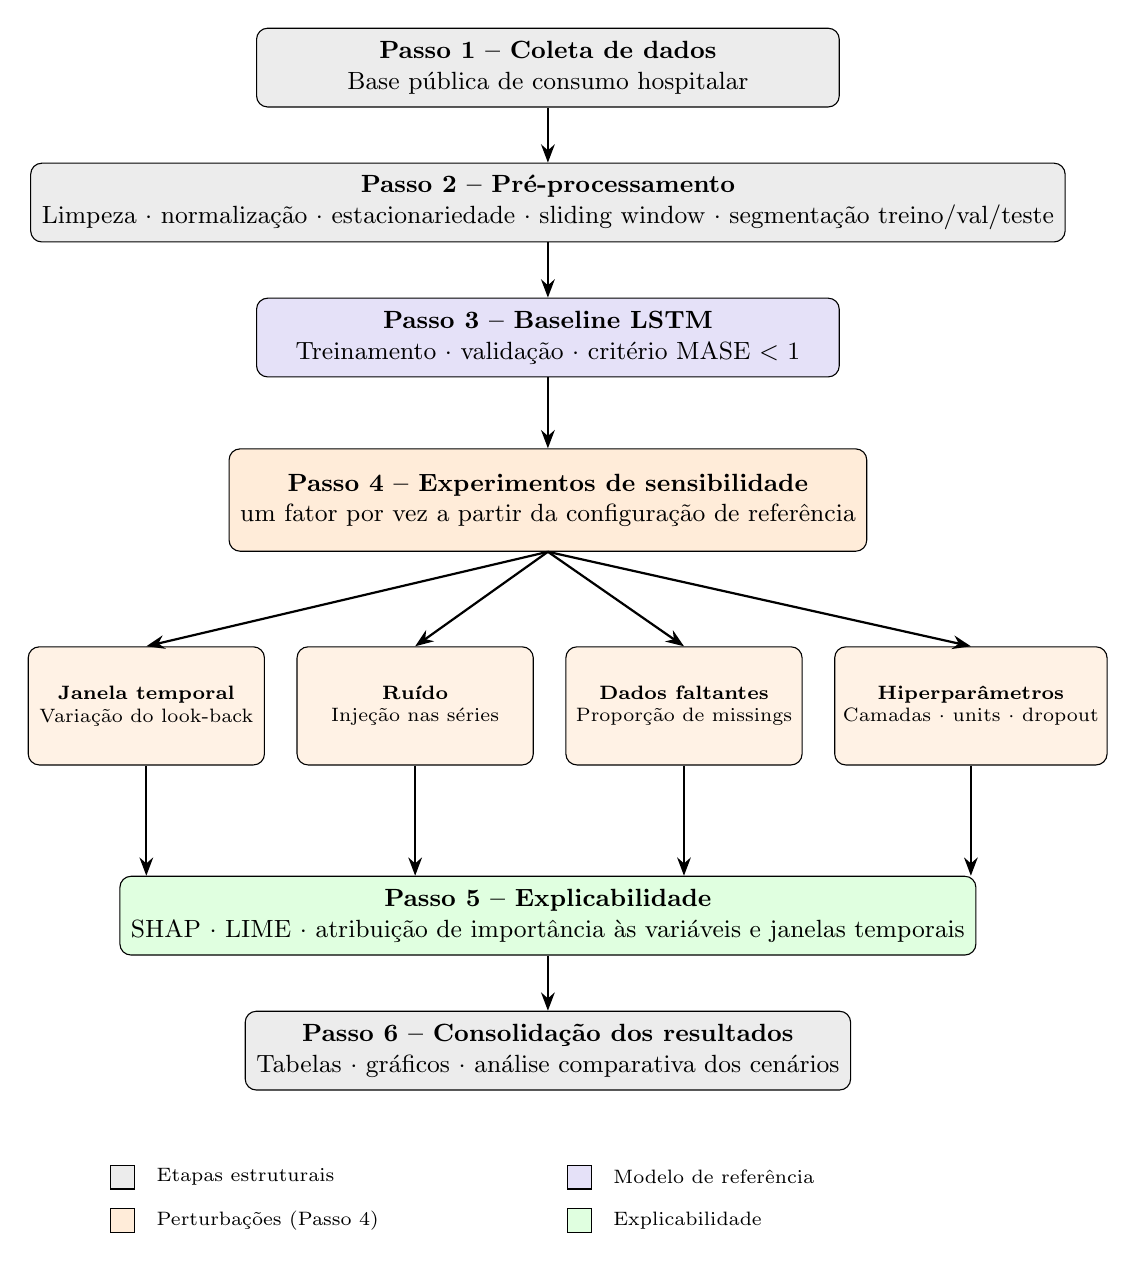
\begin{tikzpicture}[
        node distance=7mm and 6mm,
        box/.style={draw, rounded corners, align=center, minimum width=7.4cm, minimum height=1cm, font=\small, inner sep=4pt},
        subbox/.style={draw, rounded corners, align=center, minimum width=3.0cm, minimum height=1.5cm, font=\scriptsize, inner sep=3pt},
        arr/.style={-Stealth, thick}
    ]
        \node[box, fill=gray!15] (p1) {\textbf{Passo 1 -- Coleta de dados}\\Base pública de consumo hospitalar};
        \node[box, fill=gray!15, below=of p1] (p2) {\textbf{Passo 2 -- Pré-processamento}\\Limpeza $\cdot$ normalização $\cdot$ estacionariedade $\cdot$ sliding window $\cdot$ segmentação treino/val/teste};
        \node[box, fill=blue!12, below=of p2] (p3) {\textbf{Passo 3 -- Baseline LSTM}\\Treinamento $\cdot$ validação $\cdot$ critério MASE $<$ 1};
        \node[box, fill=orange!15, below=9mm of p3, minimum height=1.3cm] (p4) {\textbf{Passo 4 -- Experimentos de sensibilidade}\\um fator por vez a partir da configuração de referência};

        \node[subbox, fill=orange!10, below=1.2cm of p4, xshift=-5.1cm] (janela) {\textbf{Janela temporal}\\Variação do look-back};
        \node[subbox, fill=orange!10, right=4mm of janela] (ruido) {\textbf{Ruído}\\Injeção nas séries};
        \node[subbox, fill=orange!10, right=4mm of ruido] (faltantes) {\textbf{Dados faltantes}\\Proporção de missings};
        \node[subbox, fill=orange!10, right=4mm of faltantes] (hiper) {\textbf{Hiperparâmetros}\\Camadas $\cdot$ units $\cdot$ dropout};

        \node[box, fill=green!12, below=1.4cm of janela.south -| p4] (p5) {\textbf{Passo 5 -- Explicabilidade}\\SHAP $\cdot$ LIME $\cdot$ atribuição de importância às variáveis e janelas temporais};
        \node[box, fill=gray!15, below=of p5] (p6) {\textbf{Passo 6 -- Consolidação dos resultados}\\Tabelas $\cdot$ gráficos $\cdot$ análise comparativa dos cenários};

        \draw[arr] (p1) -- (p2);
        \draw[arr] (p2) -- (p3);
        \draw[arr] (p3) -- (p4);
        \draw[arr] (p4.south) -- (janela.north);
        \draw[arr] (p4.south) -- (ruido.north);
        \draw[arr] (p4.south) -- (faltantes.north);
        \draw[arr] (p4.south) -- (hiper.north);
        \draw[arr] (janela.south) -- (janela.south |- p5.north);
        \draw[arr] (ruido.south) -- (ruido.south |- p5.north);
        \draw[arr] (faltantes.south) -- (faltantes.south |- p5.north);
        \draw[arr] (hiper.south) -- (hiper.south |- p5.north);
        \draw[arr] (p5) -- (p6);

        \coordinate (legAnchor) at ($(p6.south)+(0,-1.1cm)$);
        \node[draw, fill=gray!15, minimum width=0.3cm, minimum height=0.3cm] at ($(legAnchor)+(-5.4cm,0)$) (leg1) {};
        \node[font=\scriptsize, anchor=west] at ($(leg1.east)+(0.15cm,0)$) {Etapas estruturais};
        \node[draw, fill=blue!12, minimum width=0.3cm, minimum height=0.3cm] at ($(legAnchor)+(0.4cm,0)$) (leg2) {};
        \node[font=\scriptsize, anchor=west] at ($(leg2.east)+(0.15cm,0)$) {Modelo de referência};
        \node[draw, fill=orange!15, minimum width=0.3cm, minimum height=0.3cm] at ($(legAnchor)+(-5.4cm,-0.55cm)$) (leg3) {};
        \node[font=\scriptsize, anchor=west] at ($(leg3.east)+(0.15cm,0)$) {Perturbações (Passo 4)};
        \node[draw, fill=green!12, minimum width=0.3cm, minimum height=0.3cm] at ($(legAnchor)+(0.4cm,-0.55cm)$) (leg4) {};
        \node[font=\scriptsize, anchor=west] at ($(leg4.east)+(0.15cm,0)$) {Explicabilidade};
    \end{tikzpicture}
    \caption{Pipeline experimental proposto para análise de sensibilidade do modelo LSTM}
    \label{fig:pipeline}
\end{figure}

\subsection{Tecnologias e ferramentas}
\label{subsec:tecnologias}

A implementação será realizada em linguagem Python, pela maturidade de seu ecossistema para aprendizado de máquina e por sua adoção nos trabalhos relacionados analisados. Para a construção e o treinamento do modelo LSTM, prevê-se o uso de Keras, utilizado por \citeonline{AGARWAL2024979}. O pré-processamento e o cálculo de métricas apoiam-se nas bibliotecas scikit-learn (normalização e métricas), pandas e NumPy (manipulação de dados). As análises de explicabilidade utilizarão as bibliotecas SHAP e LIME, e a visualização dos resultados, Matplotlib e Seaborn. Para etapas opcionais de decomposição de séries (por exemplo, STL), pode-se recorrer ao statsmodels.

A experimentação será conduzida em ambiente de máquina local: Intel(R) Core(TM) i5-14600KF (3,50 GHz) CPU; 16,0 GB RAM; NVIDIA GeForce RTX 5060 (8 GB) GPU, com versionamento das dependências e fixação de sementes aleatórias, de modo a garantir a reprodutibilidade dos experimentos e o controle sobre fatores externos ao modelo, conforme previsto no objetivo secundário 3 (Seção~\ref{sec:objetivos_secundarios}).

\subsection{Funcionalidades principais}
\label{subsec:funcionalidades}

As funcionalidades do pipeline, alinhadas aos objetivos do trabalho, são: treinar e avaliar um modelo LSTM de referência para previsão de demanda de itens críticos; executar experimentos de perturbação controlada sobre parâmetros de entrada e hiperparâmetros; mensurar a variabilidade das métricas de desempenho frente a cada perturbação; gerar, por meio de SHAP e LIME, a importância das variáveis e dos instantes temporais nas previsões; e consolidar os resultados em tabelas e gráficos que permitam comparar os cenários e identificar os fatores de maior influência.

\subsection{Metodologia de desenvolvimento}
\label{subsec:metodologia_dev}

Adota-se uma abordagem experimental e incremental. O desenvolvimento parte da construção do pipeline de dados e do modelo de referência (baseline); somente após a validação do baseline os experimentos de sensibilidade são executados, um fator por vez a partir da configuração de referência, de modo a isolar o efeito de cada variação. Essa estratégia evita a explosão combinatória de cenários e mantém a interpretabilidade dos resultados. O ciclo de trabalho é iterativo: cada experimento é executado, registrado e analisado antes do planejamento do seguinte, em consonância com a recomendação da literatura de integrar a avaliação de desempenho ao longo de todo o fluxo, e não apenas à etapa final.

\subsection{Critérios de validação}
\label{subsec:criterios_validacao}

O sucesso da solução será avaliado em duas frentes. Na primeira, relativa à qualidade do modelo de referência, espera-se que o baseline apresente desempenho superior ao de um preditor ingênuo, critério verificável por meio do MASE, considerado satisfatório quando inferior a 1. Na segunda frente, relativa ao objetivo central do trabalho, a validação se dá pela própria análise de sensibilidade: a solução será considerada bem-sucedida se permitir quantificar de forma sistemática a variação das métricas (MAE, RMSE, MAPE e MASE) sob cada perturbação, identificar quais parâmetros exercem maior influência sobre o desempenho preditivo e caracterizar os cenários que representam maior risco para a aplicação prática em ambientes hospitalares. A consistência dos resultados será reforçada pela fixação de sementes aleatórias e pela repetição das execuções, de modo a distinguir o efeito das perturbações do ruído decorrente da inicialização do modelo.

% ---------------------------------------------------------------
\section{Conjunto de dados}
\label{sec:conjunto_dados}

O primeiro candidato a ser utilizado neste trabalho é de natureza pública e contém registros de posicionamento de estoque da rede pública de saúde do Brasil. A base contempla variáveis como data, nome do medicamento, quantidade em estoque, categoria terapêutica e outras informações relevantes para a previsão de demanda, tendo sido selecionada pela sua disponibilidade aberta e pela capacidade de conferir validade e reprodutibilidade aos resultados obtidos.

Com o objetivo de concentrar a análise em itens de maior relevância para o sistema de saúde, a base será tratada de forma a resultar em um grupo de medicamentos essenciais, conforme definido pela RENAME \citeonline{RENAME2024}. A seleção desses itens foi orientada por critérios de impacto assistencial e relevância epidemiológica, com ênfase em medicamentos voltados ao aparelho respiratório, cuja gestão eficiente é crucial para o atendimento adequado à população. Ao todo, cinco medicamentos compõem esse grupo de itens críticos, os quais serão detalhados no capítulo de desenvolvimento, juntamente com a descrição das variáveis selecionadas e o processo de pré-processamento aplicado.
% TODO(Gabriel): a frase "Fonte dos dados: Fonte dos dados." abaixo está circular/incompleta
% no PDF original -- substituir pelo nome e link reais do portal/API (ex.: BNAFAR/HORUS-DEMAS,
% Ministério da Saúde) assim que a questão de acesso à base for resolvida.
Fonte dos dados: Fonte dos dados.

O segundo candidato a ser utilizado neste trabalho também é de natureza pública e aberta, sendo composto por registros históricos de vendas de medicamentos extraídos do sistema de ponto de venda (Point-of-Sale) -- tecnologia de caixa que pequenas empresas utilizam para aceitar pagamentos e controlar as vendas -- utilizado por uma rede farmacêutica. A base abrange seis anos de operação (2014--2019) e contempla aproximadamente 600 mil transações referentes a 57 medicamentos, organizados segundo o Sistema de Classificação Anatômico-Terapêutico-Químico (ATC) em oito categorias terapêuticas \citeonline{ATCDDD2026}. Entre as variáveis disponíveis encontram-se a data (e, em sua granularidade original, o horário) da venda, o nome do medicamento, a categoria terapêutica e a quantidade comercializada, esta última empregada como sinal direto de demanda. Os dados são ainda disponibilizados em diferentes granularidades temporais horária, diária, semanal e mensal, o que confere flexibilidade à definição da janela de previsão. A base foi selecionada por sua disponibilidade aberta sob licença Creative Commons, por sua aplicação consolidada na literatura de previsão de demanda farmacêutica \citeonline{Zdravkovic2020} e pela capacidade de conferir validade e reprodutibilidade aos resultados obtidos.

À semelhança do tratamento previsto para o primeiro candidato, a análise será concentrada em itens de maior relevância assistencial, com ênfase em medicamentos voltados ao aparelho respiratório. Para tanto, serão privilegiadas as categorias ATC associadas ao sistema respiratório R03 (medicamentos para doenças obstrutivas das vias aéreas) e R06 (anti-histamínicos de uso sistêmico), das quais será derivado o grupo de itens críticos a ser detalhado no capítulo de desenvolvimento, juntamente com a descrição das variáveis selecionadas e o processo de pré-processamento aplicado.
% TODO(Gabriel): idem acima -- referenciar diretamente a fonte (Kaggle/Zdravković, já citado)
% em vez de repetir o placeholder circular.
Fonte dos dados: Fonte dos dados.

% ---------------------------------------------------------------
\section{Cronograma de trabalho}
\label{sec:cronograma}

O cronograma a seguir apresenta, no formato de diagrama de Gantt, as atividades previstas para o desenvolvimento do TCC2, distribuídas ao longo das semanas do semestre.

% TODO(Gabriel): as datas exatas de cada barra não puderam ser recuperadas do PDF (o texto
% extraído de um gráfico não preserva a posição numérica das barras). A distribuição abaixo
% é uma reconstrução plausível, alinhando os 7 módulos do pipeline às semanas 5-12; ajuste
% conforme o cronograma original se ele diferir.
\begin{figure}[htb]
    \centering
    \caption{Cronograma de atividades -- Diagrama de Gantt}
    \label{fig:gantt}
    \begin{ganttchart}[
        hgrid,
        vgrid,
        x unit=0.72cm,
        y unit title=0.6cm,
        y unit chart=0.65cm,
        title height=1,
        bar height=0.5,
        bar label font=\scriptsize,
        title label font=\small,
        milestone label font=\scriptsize\itshape,
        group label font=\scriptsize\bfseries,
        bar/.append style={fill=blue!40},
        group/.append style={draw=black, fill=blue!70},
        milestone/.append style={fill=red!70},
    ]{1}{16}
        % Título: semanas de 1 a 16
        \gantttitle{Semanas}{16} \\
        \gantttitlelist{1,...,16}{1} \\

        % Grupo 1: Planejamento
        \ganttgroup{Fase 1: Planejamento}{1}{4} \\
        \ganttbar{Revisão bibliográfica}{1}{3} \\
        \ganttbar{Definição de requisitos}{2}{4} \\
        \ganttbar{Projeto da arquitetura}{3}{4} \\
        \ganttmilestone{Entrega do projeto}{4} \\

        % Grupo 2: Desenvolvimento (um bloco por módulo do pipeline)
        \ganttgroup{Fase 2: Desenvolvimento}{5}{12} \\
        \ganttbar{Módulo de aquisição e pré-processamento}{5}{6} \\
        \ganttbar{Módulo de definição do modelo}{6}{7} \\
        \ganttbar{Módulo de treinamento}{7}{8} \\
        \ganttbar{Módulo de avaliação}{8}{9} \\
        \ganttbar{Módulo de experimentos de sensibilidade}{9}{10} \\
        \ganttbar{Módulo de explicabilidade}{10}{11} \\
        \ganttbar{Módulo de registro e análise de resultados}{11}{12} \\
        \ganttmilestone{Protótipo funcional}{12} \\

        % Grupo 3: Testes e Finalização
        \ganttgroup{Fase 3: Validação}{13}{16} \\
        \ganttbar{Testes e validação}{13}{14} \\
        \ganttbar{Ajustes e correções}{14}{15} \\
        \ganttbar{Redação final do TCC2}{13}{16} \\
        \ganttmilestone{Entrega final}{16}

        % Ligações entre atividades
        \ganttlink{elem2}{elem3}
        \ganttlink{elem3}{elem4}
        \ganttlink{elem4}{elem5}
        \ganttlink{elem7}{elem8}
        \ganttlink{elem8}{elem9}
        \ganttlink{elem9}{elem10}
        \ganttlink{elem10}{elem11}
        \ganttlink{elem11}{elem12}
        \ganttlink{elem12}{elem13}
        \ganttlink{elem13}{elem14}
        \ganttlink{elem16}{elem17}
    \end{ganttchart}
    \legend{Fonte: Elaborado pelo autor (2025)}
\end{figure}

% ---------------------------------------------------------------
% ELEMENTOS PÓS-TEXTUAIS
% ---------------------------------------------------------------
\postextual

% ===============================================================
% CAPÍTULO 4 - REFERÊNCIAS BIBLIOGRÁFICAS
% ===============================================================
% As referências bibliográficas são geradas automaticamente a partir
% do arquivo bibliografia.bib, seguindo o padrão ABNT (NBR 6023).
%
% COMO CITAR no texto:
%   \cite{chave}         -> (SOBRENOME, ano) — citação indireta
%   \citeonline{chave}   -> Sobrenome (ano) — citação direta no texto
%
% Veja o arquivo bibliografia.bib para exemplos de cada tipo.
% ---------------------------------------------------------------
\bibliography{bibliografia}

% ---------------------------------------------------------------
% APÊNDICES (se necessário)
% ---------------------------------------------------------------
% \begin{apendicesenv}
% \partapendices
%
% \chapter{Nome do Apêndice}
% \label{ap:apendice1}
%
% Conteúdo do apêndice (material elaborado pelo próprio autor).
%
% \end{apendicesenv}

% ---------------------------------------------------------------
% ANEXOS (se necessário)
% ---------------------------------------------------------------
% \begin{anexosenv}
% \partanexos
%
% \chapter{Nome do Anexo}
% \label{an:anexo1}
%
% Conteúdo do anexo (material de terceiros).
%
% \end{anexosenv}

\end{document}